\documentclass[conference]{IEEEtran}
\IEEEoverridecommandlockouts
% The preceding line is only needed to identify funding in the first footnote. If that is unneeded, please comment it out.
\usepackage{cite}
\usepackage{amsmath,amssymb,amsfonts}
\usepackage{algorithmic}
\usepackage{graphicx}
\usepackage{textcomp}
\usepackage{xcolor}
\def\BibTeX{{\rm B\kern-.05em{\sc i\kern-.025em b}\kern-.08em
    T\kern-.1667em\lower.7ex\hbox{E}\kern-.125emX}}
\begin{document}

\title{Real-time Thrust Estimation and Regulation for Multirotor Aerial Vehicle\\
{}
\thanks{}
}

\author{\IEEEauthorblockN{1\textsuperscript{st} Adithya Ravishankara}
\IEEEauthorblockA{\textit{dept. name of organization (of Aff.)} \\
\textit{name of organization (of Aff.)}\\
City, Country \\
email address}
\and
\IEEEauthorblockN{2\textsuperscript{nd} Bara Emran}
\IEEEauthorblockA{\textit{dept. name of organization (of Aff.)} \\
\textit{name of organization (of Aff.)}\\
City, Country \\
email address}
\and
\IEEEauthorblockN{3\textsuperscript{rd} Sherman}
\IEEEauthorblockA{\textit{dept. name of organization (of Aff.)} \\
\textit{name of organization (of Aff.)}\\
City, Country \\
email address}
\and
\IEEEauthorblockN{4\textsuperscript{th} Homayoun Najjaran}
\IEEEauthorblockA{\textit{dept. name of organization (of Aff.)} \\
\textit{name of organization (of Aff.)}\\
City, Country \\
email address}

}

\maketitle

\begin{abstract}
In this paper, we present a real-time approach to sense and regulate the thrust produced by rotors with fixed-pitch blade commonly used on multirotor aerial vehicles (MAV). The proposed schemes consist of integrating a wind sensor mounted onboard to measure the wind speed generated by the rotor directly. The wind measurement is then used with a simple control system and effective estimation algorithms to perform a precise controlling of the rotor thrust in real time. This integration significantly improves the disturbance rejection and fault estimation of the thrust and rotor, respectively. Specifically, a direct regulation of the thrust will improve the MAV systems performance while performing aggressive maneuvers or when subjected to external disturbances. Moreover, this approach can be employed to estimate the effective loss of a rotor for fault-tolerant control systems. The features of the proposed approach are demonstrated using a testbed and compared to a classical electrical speed control. Different experiments were performed to validate the efficiency of the proposed approach in maintaining the thrust in the presence of a wind gust and rotor efficiency loss.
\end{abstract}

\begin{IEEEkeywords}
Sensor,Control,Kalman,Quadrotor
\end{IEEEkeywords}

\section{Introduction}
Unmanned aerial vehicles (UAV), especially multirotor, have become quite commonplace in many industries ranging from inspection, racing to military applications \cite{bara}, \cite{Mathe}. Over the past decade, there has been an incredible amount of research and advancement within this field leading to its proliferation and allowing for the technology to become more accessible. One of the major areas of research regarding UAV is the control system that directs the motor-rotor system. The control mechanism ranges in complexity from the common motor-rotor control to a more complex system that takes into consideration parameters such as thrust or torque. The control of the motor-rotor has to account for different external and internal factors, such as the ambient wind speed, the rotation speed of the propeller (RPM), the pitch of the propeller and the internal loops of the Electronic Speed Controller (ESC). Typically, rotor control systems in UAV are operated in open control loops. That is, the flight controller (FC) sends the desired speed value to the ESC that applies a particular voltage to the motor based on previously calibrated settings. The ESC uses the feedback signals of the rotor’s current and voltage to maintain its desired speed. In this method, however, the thrust generated by the propeller spinning is unknown to the FC. Recently, advanced FC employs static aerodynamic models relating rotor speed to estimate and control the generated thrust. Usually, these models are obtained after intensive experiments performed in static-free air environment to detrain the motor’s and propeller’s characteristics. However, when the system is subjected to a disturbance, these models become inaccurate. These external disturbances could accrue due to wind or when the vehicle is performing an agile maneuver. Thus, the lack of a direct measurement of the actual thrust is attracting the interest of the robot community recently. In this paper, we focus on determining a type of sensor that can efficiently measure the generated thrust of a propeller to use it for controlling the UAV. This allows for a smarter and more robust control system.

There has been an enormous strive to develop methods to obtain a closed loop control system for UAVs. The methods range from thrust modeling to estimation using different sensors. The majority of the estimation-based controls rely on the voltage or current drawn by the motors.
Awan et. al. \cite{awan} developed an adaptive observer-based thrust estimation system. This method allowed the MAV to maintain a hover with higher precision compared to previous methods involving thrust estimation. However, their proposed structure only accounts for hovering condition and the models were based around a linearized system. As a result, the system was highly violable for disturbances. This was accounted in Sydney et. al. \cite{sydney}, where they have proposed a highly complex estimation system and considered the nonlinear model of the system. Similarly, Mahoney et. al. \cite{mahoney1} devised a system which estimates the thrust using an iterative based calculation. This system while it allows for a valid estimation of the thrust, it is relatively complex and requires heavy computation. Letter in Mahony (2017), they have improved the estimation algorithm using the feedback signal of the voltage and current given to the motor by the ESC. Their system works to maintain a thrust given some disturbance. Still, their system runs through an iterative loop before detecting an appropriate response to extraneous forces. This system while it allows for a robust estimation of the thrust, it is still a complex system. As well their method requires a significant amount of calibration for both the propellers and rotors which makes it harder to employ in different systems. Streit \cite{str} developed a control system to compensate for wind disturbances using a pitot-tube sensor along with an accompanying estimation algorithm. While this seems similar to the Yeo et al paper, there are some major differences. Streit has only one pitot sensor onboard the UAV which is unidirectional and therefore only applies to forward motion. As well the pitot-tube is made of brass and therefore not feasible for all smaller UAV’s as it will be too heavy. Yeo et al have used fabricated pitot tubes placed below each propeller to measure the rotor downwash and compare them to the estimated expected wind speed. Their system is ultimately used to localize external noise from other UAV’s and therefore an exceedingly accurate measurement is not as important. While the sensor can accurately measure wind speed accurately during vertical motion, there is a significant divergence from the ground speed measurement during lateral movement. As well there is a very limited range of speeds that are available for measurement from the probe.


\section{2}
\subsection{Wind sensor math/theory}
We have to start by defining the three different velocities that apply to a propeller.\\
\begin{eqnarray}
\label{e1}
v_x , v_y , v_z \\
\label{e2}
v^s_{x} , v^s_{y} , v^s_{z} \\
\label{e3}
v^i_{x} , v^i_{y} , v^i_{z}
\end{eqnarray}
Where \ref{e1} Is the velocity of the drone, the body frame velocity, \ref{e2} is the velocity of the wind approaching the propellers, the stream velocity, and \ref{e3} is the induced velocity of the propellers.\\
Since we are doing only the static tests in this paper, we can disregard the horizontal components of the wind as well as the body frame velocities. Then we can state 
\begin{eqnarray}
\nonumber
v_s = v^s_{z}\\
\nonumber
v_i = v^i_{z}
\end{eqnarray}
As well, since we have stationary system, the frame velocities can be ignored as well. What the wind sensor will notice is 
\begin{equation}
v_{tot} = v_{i} + v_{s}
\label{vtot}
\end{equation}	
Generally, when no disturbances are applied we can assume that $v_s$ is $0$ as a means of simplifying our system.
Modern Device \cite{md} gives us the equation 
\begin{eqnarray}
WS = \frac{(V - V_{z})*0.087288}{3.038517 * T_{c} ^{0.115157}} ^ {3.009364}
\label{wind_speed}
\end{eqnarray}
Where $WS$ is the wind speed,in miles/hour, $V$ is the measured voltage, $V$ is the calibrated voltage when there is no wind, and $T_c$ is the current temperature in celsius which is also measured by the sensor. While the basis of this paper is around the wind speed, it is not important to know the exact wind speed and therefore throughout the rest of our calculations, we only consider the measured voltage. 
%How does wind speed relate to voltage
To explain the relation of wind to thrust, let's radically simplify it and assume it is a linear system.  With this being the case, it can be stated that 
\begin{equation}
F_p= \frac{\partial p}{\partial t}
\label{fvm}
\end{equation}
where $F_p$ is the force the propeller exerts, $p$ is momentum and $t$ is time. From this we can expand this to 
\begin{eqnarray}
F_p= \frac{mv_{tot} - mv_{s}}{\Delta t}\\ 
\label{fvm2}
F_p= m*(v_{tot}-v{s}) 
\label{fvm3}
\end{eqnarray}
where $m$ is the mass of air flowing. Then making the assumption that $\Delta t = 1$ we get \ref{fvm3}.	Now to consider the efficiency of the propeller we can say 
\begin{eqnarray}	
v_{i}\prime = v_{i}* \gamma\\
v_{tot}\prime = v_i\prime + v_s
\label{eff}
\end{eqnarray}
where $\gamma$ is some efficiency factor where $0 \leq  \gamma \leq 1$ which degrades as the stream velocity $v_s$ approaches $v_i$\cite{someone}. In doing so we can assume that for a non-zero $v_s$ 
\begin{equation}
F_p\prime < F_p
\end{equation}
This is the reasoning behind why as winds buffet a drone mid-flight, the drone's thrust vector tends to drop. Hence we can measure this change in thrust and correct for it.
\subsection{Adaptive Fuzzy Kalman Filter }

Accurate a priori information of the measurement and process noise statistical matrices of the state estimator is needed to avoid the divergence of the filter [3], [4]. To resolve the problem of having imperfect a priori information, adapting R and/or Q matrices was introduced using several adaptive estimation techniques [5]–[7]. Among these, the Innovative-based Adaptive Estimation (IAE) and Multiple Model Adaptive Estimation (MMAE) are commonly utilized to adapt the Kalman filter. Incorporating the rules of fuzzy logic to adjust the variances of these matrices has been studied in several research works. The Adaptive Fuzzy Kalman Filter q (AFKF) has been designed to improve the performance of the conventional filter in rejecting the measurement noise and estimating the navigational states accurately [8], [9]. 
The recurrent adjustment process of the variances of the statistical matrices Rk is designed based on an IAE approach. This approach is based on a covariance-matching algorithm which examines the degree of the mismatch DoM between the actual covariance $v_{K+1}$ of the residual with its theoretical value $S_{K+1}$. 
\begin{equation}
DoM = S_{k+1} - C_{k+1}
\label{dom}
\end{equation}
After calculating DoM, a Fuzzy Inference System (FIS) has been tuned to compute the adjustment of the measurement noise matrix $R_{k+1}$ and update the matrix at each cycle of state estimation.
\begin{equation}
R_{k+1} = R_k +\delta R_{K+1}
\label{rk1}
\end{equation} 
	\section{3}
\subsection{RCBenchmark Thrust Stand Dynamometer}
%THE THRUST STAND
In our setup we used a thrust stand obtained from RCBenchmark, specifically the RCBenchmark Thrust stand and Dynamometer Series 1580 \cite{rcb} as our testbed. The measurements from the thrust stand will be our "ground truth". This thrust stand incorporates a micro-controller board along with three, three-axis strain guage to measure the forces and the torque derived by the propeller. The board also collects data on the voltage, current and the signal to the ESC's which allows us to measure the power draw of the motor, and the RPM of the motor. Along with this there is an associated GUI which allows us to control the board and collect and visualize the data. The testbed collects data at a very high rate of close to 1kHz but then averages the data to eliminate outliers, so the data rate is 40Hz. This is more than adequate for the purposes of modeling the thrust response of the propeller to various stimuli. 
\subsection{Modern Device Wind Sensor}
The wind sensor we have chosen to use is the "Modern Device- Wind Sensor Rev. P" \cite{md}. This device is a hot wire anemometer that is designed to measure wind from any direction. Hot wire anemometers work by passing a constant current through a thin wire which heats up due to the current. As the wind flows past the wire, the wire will be cooled down rapidly, resulting in a change in the measured voltage, which is the value that we observe \cite{hot_wire}. This system allows us to measure the wind speed that is resultant of the propeller. 
To understand the limitations of the wind sensor, we performed a series of tests to characterize the sensor. The first of which was to determine under which orientation the sensor observed the highest range of wind speeds. As seen in \ref{orient_test}, the orientation of placing the wind sensor normal to the direction of wind flow allowed for the highest range of measurement. Next we performed a test to determine the feasible range of measurement. This was done by exposing the wind sensor to a step-signal test and a pulse signal test ranging from the minimal PWM value to approximately $50\%$ of the motor's max value, the results of which are in \ref{min_max}. The PWM values in this case are based around the Simulink-Arduino Library PWM module.  This resulted in a working range from $PWM = 44$ to $PWM = 60$. While there is possibility for the wind sensor to measure higher wind speeds, there is a significant amount of noise even with the addition of a low-pass filter, hence we decided to limit the max speed of our experiment. 
Another factor that we deem is important to characterize is the speed of response to change of wind speed. We measured this by running the propeller at various different speeds, while tracking the thrust output on the testbed as our base measurement of response time and then comparing the response time to see the lag in response time. By doing this we found that there was a negligible lag time of less than $10 ms$, which is our resolution for each measurement.
Lastly we measured the location of the wind sensor in relation to the propellers. To do so we measured a semi-circle area behind the propeller to deem the location of highest wind sensitivity. Resulting in a map as seen in figure \ref{area}. 
By characterizing the wind sensor, we can ensure that it is in the optimal configuration for us to collect data.
\section{Results}
\subsection{Experimental Setup- How we set up the kalman/Algorithm}

We developed a control architecture as pictured in fig \ref{block_diagram} where there are two sources of measurement for the thrust value. the primary value is from the wind sensor which is measured through an Arduino. The voltage value that the arduino measures is then converted to a thrust value through the power function
\begin{equation}
Thrust = 4.701 * 10^{15} * V_w^{6.146} + 0.0731
\label{wind_power}
\end{equation}
The secondary measurement of thrust is a polynomial function that converts the output PWM value that is used to control the propeller. \newline
\begin{eqnarray}
Thrust = 1.957*10^{-5}*PWM^4 \\
- 7.476*10^{-4}*PWM^3 \nonumber\\ 
+ 1.272*10^{-2}*PWM^2 \nonumber\\
+ .01092*PWM - .01842 \nonumber
\label{pwm_poly}
\end{eqnarray}
These values are then passed through a Kalman Filter weighted towards the wind sensor. This method allows for the system to accurately determine the thrust value output while reducing noise due to the nature of the wind. Next this value is passed to a PI controller which generates the appropriate response for the error between desired and measured. 
\subsection{The tests}
Figures \ref{akf1},\ref{akf2} demonstrate the thrust estimation using the conventional and the adaptive fuzzy state estimation techniques. As can be seen, the proposed AFKF has exhibited better performance in terms of rejecting the noise associated with the measurement compared to the classical KF. Figures \ref{akf1},\ref{akf2} presents the estimation errors of the position states. The AFKF shows lower magnitudes of estimation error compared to these of the KF. 

To ensure the viability of our algorithm and if it would respond to external stimuli the way we expected, we performed several tests that caused significant errors in the propeller's response. The first test that we ran was to measure the response of the kalman filter and ensure that our thrust calculation was accurate in relation to the testbed recorded thrust. As seen in fig \ref{kalman} the kalman filter, while noisy due to the wind variations in the wind sensor data, follows the thrust value from the testbed closely. This result gives us the confidence to setup the PI based on the kalman filter's value. 
To ensure the functionality of the controller we set up several faults and disturbances to test the response of the system. The first step was to create an external disturbance by placing another propeller and blowing wind perpendicular to the axis of the main propeller. This would be akin to horizontal crosswind flow across the propeller.

Based on the results of fig \ref{wind_disturb}, the control algorithm can determine the appropriate correction for such a disturbance through

\subsection{Shortcomings and limitations}
As mentioned previously, having a closed loop system allows for a more robust and agile system which allows for better flight performance. Some of the application for this level of performance include a better landing algorithm, proximity detection of other MAV's, more sophisticated hovering control, fault detection, and fault tolerance. These areas would all benefit by having a physical measurement of the thrust rather than an estimation.

There are certain limitations within our setup that we have to address. The first of which is the low range of the wind sensor which can maximally measure only $25\%$ of the motor's maximum RPM. The other major shortcoming of our paper is the static nature of the experiments. Our tests have only been in a fixed and controlled environment, with only one motor as the test. In real situations on a quadrotor or such, the behaviour of our system might be significantly different.  	
low wind speed. Have not accounted for multiple sources of wind. fixed and controlled environment. only one propeller. 
\section{5}
\subsection{Reiteration of results}
In this paper we presented a closed loop control system for the purposes of controlling MAV rotor systems by the introduction of a hot wire anemometer. The anemometer measures the rate of wind flow from the downwash of the MAV rotor and there is a linear relationship that is developed between wind flow velocity and the thrust output of the system. Through this relationship we developed a PI controller that maintains a desired thrust value against internal and external disturbances.
\subsection{Reiteration of applications}

\subsection{}
	\begin{figure}[htbp]
	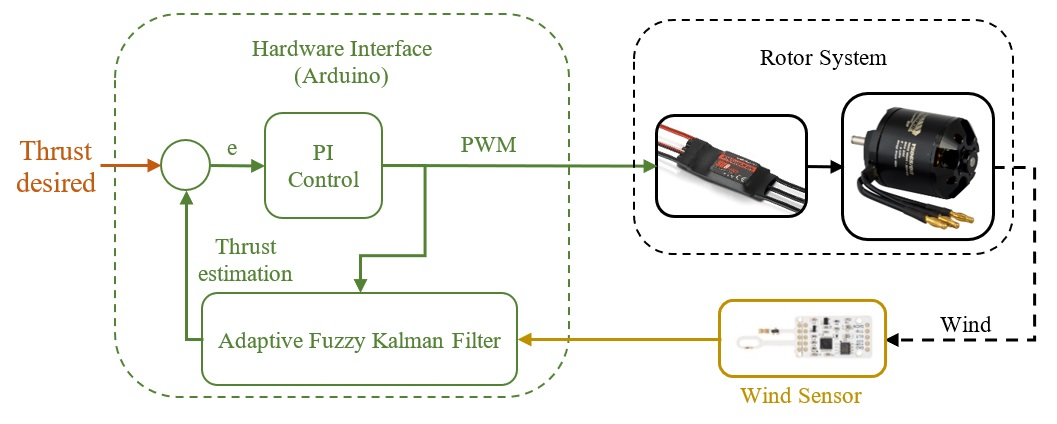
\includegraphics[width=7cm]{images/Figure_2/Block Diagram.jpg}
	\caption{Block Diagram}
	\label{block_diagram}
	\end{figure}
	\begin{figure}[htbp]
	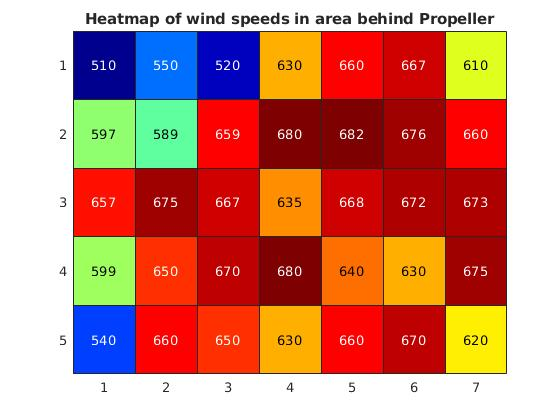
\includegraphics[width=10cm]{images/figure_1/area_heatmap.jpg}
	\caption{Block Diagram}
	\label{area}
	\end{figure}
	\begin{figure}[htbp]
	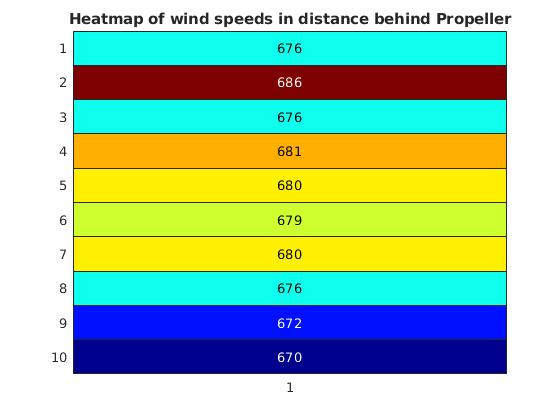
\includegraphics[width = 7cm]{images/figure_1/dist_heatmap.jpg}
	\caption{Block Diagram}
	\label{dist}
\end{figure}
	\begin{figure}[htbp]
	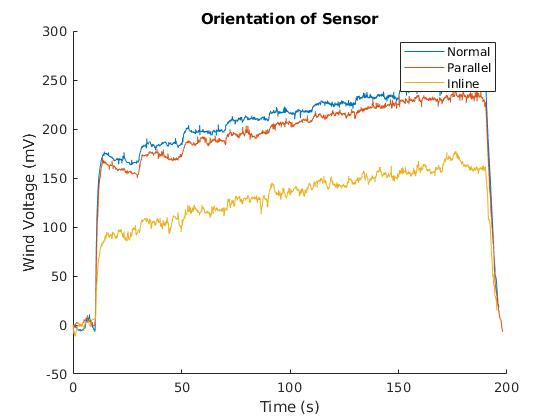
\includegraphics[width=10cm]{images/figure_1/orientation.jpg}
	\caption{Block Diagram}
	\label{orientation}
\end{figure}
	\begin{figure}[htbp]
	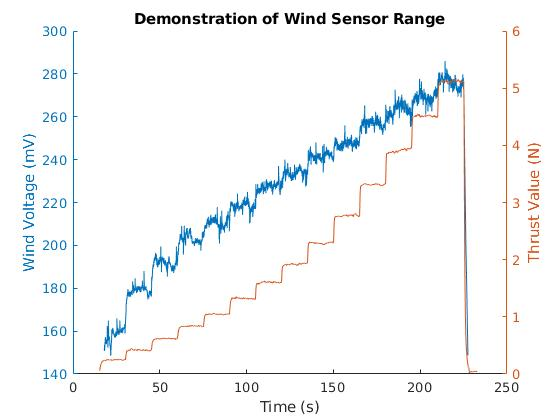
\includegraphics[width=10cm]{images/figure_1/range.jpg}
	\caption{range}
	\label{range}
\end{figure}
	\begin{figure}[htbp]
	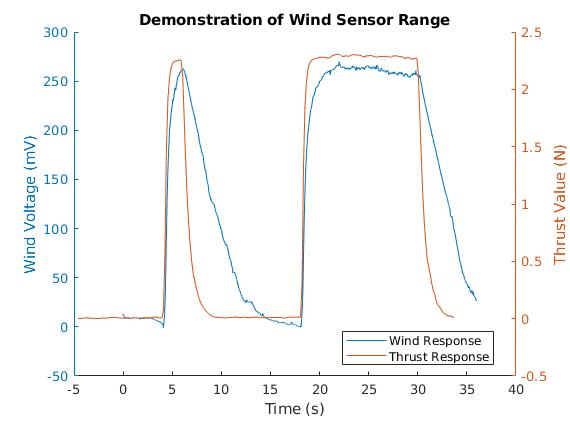
\includegraphics[width=10cm]{images/figure_1/response.jpg}
	\caption{response}
	\label{response}
\end{figure}
\begin{figure}[htbp]
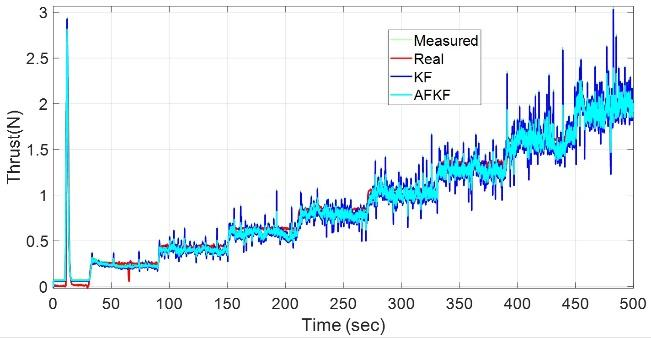
\includegraphics[width=10cm]{images/akf1.jpg}
\caption{response}
\label{akf1}
\end{figure}
\begin{figure}[htbp]
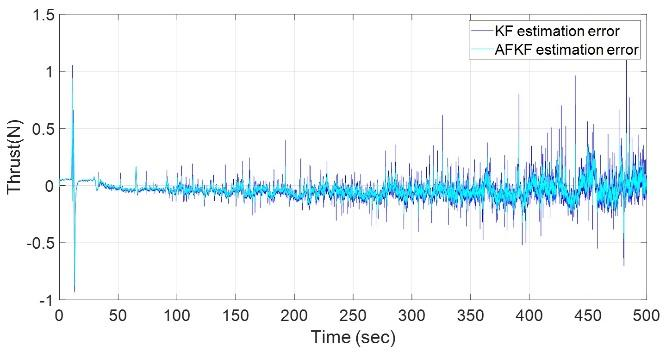
\includegraphics[width=10cm]{images/akf2.jpg}
\caption{response}
\label{akf2}
\end{figure}
\begin{figure}[htbp]
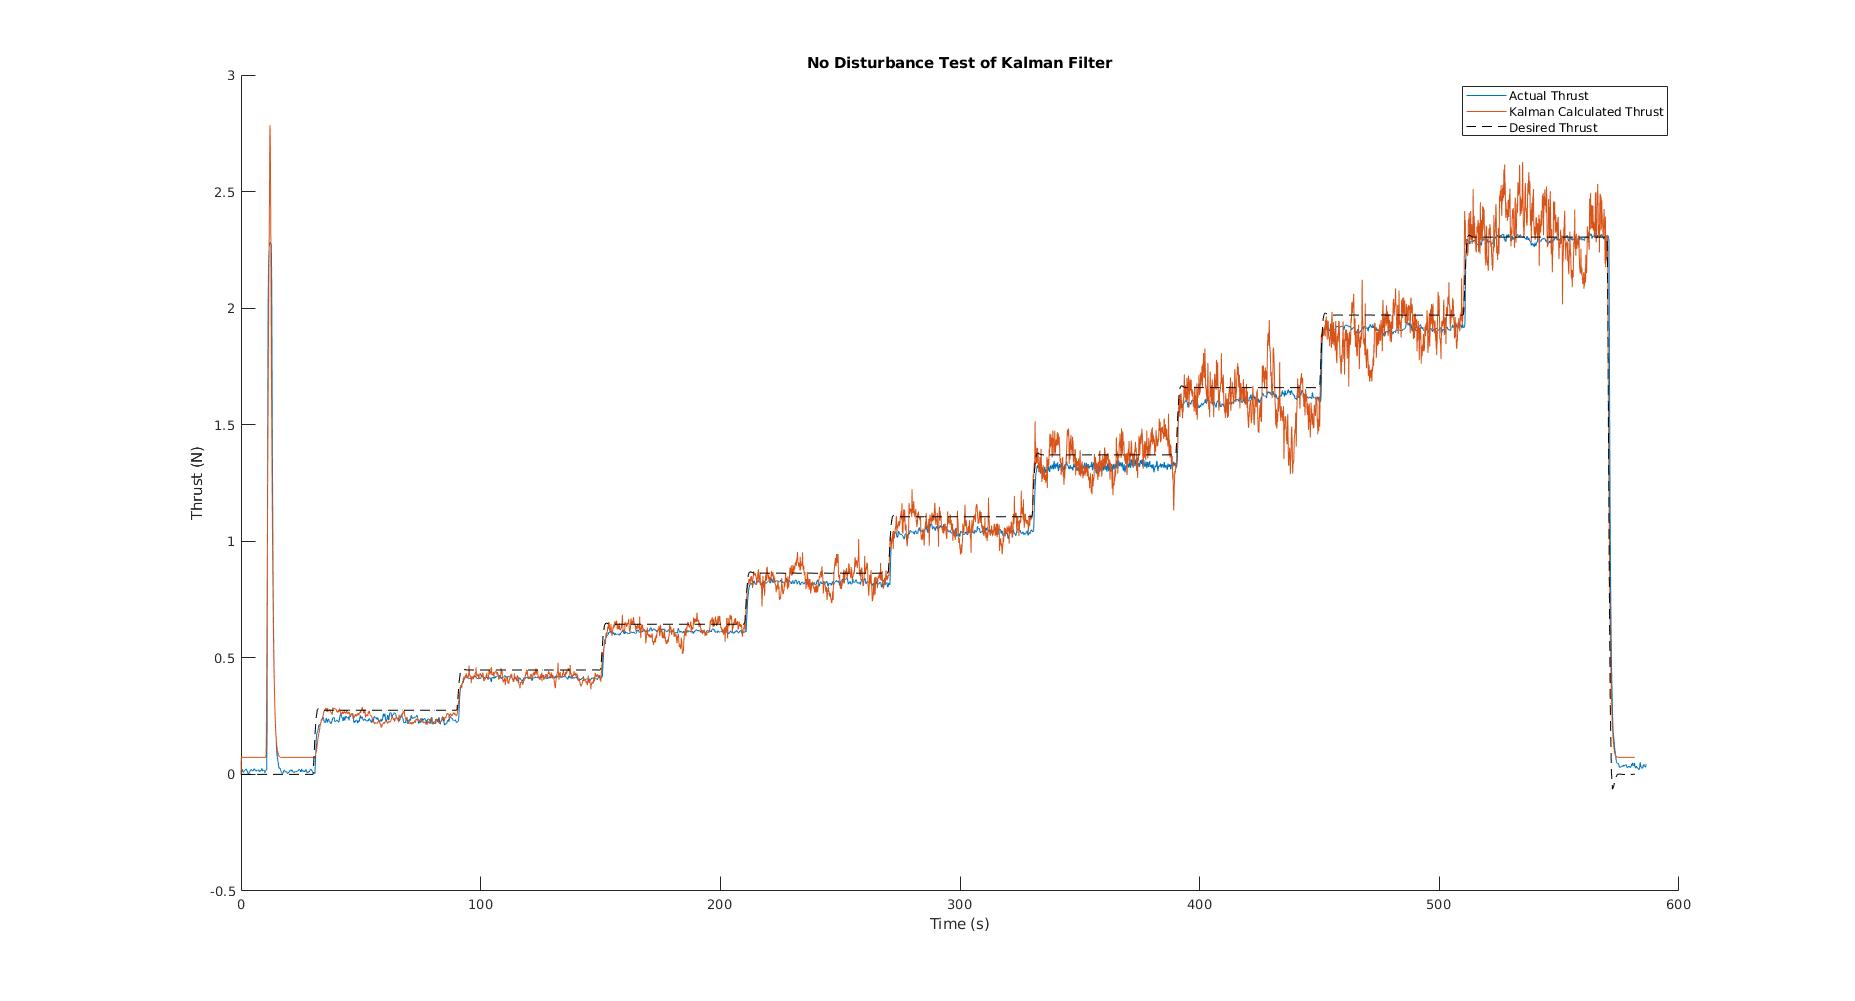
\includegraphics[width=10cm]{images/Figure_2/kalman.jpg}
\caption{response}
\label{kalman}
\end{figure}
\begin{figure}[htbp]
	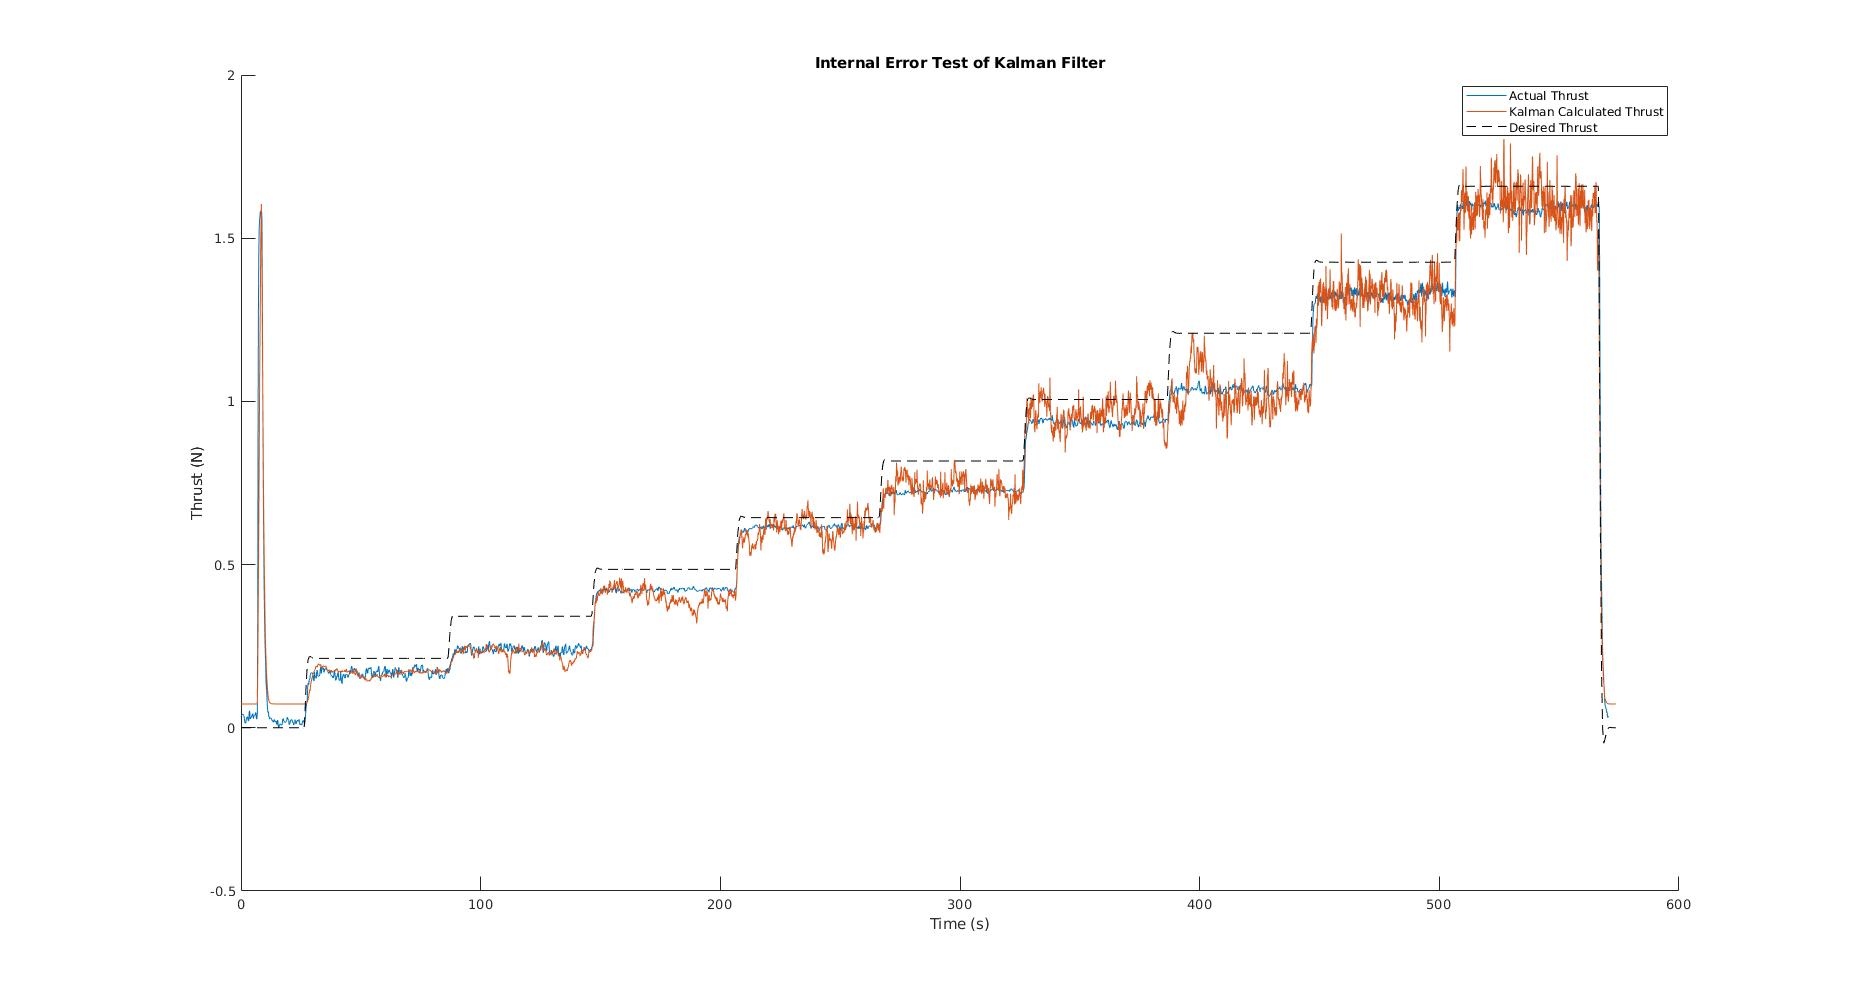
\includegraphics[width=10cm]{images/Figure_2/pwm_reduc.jpg}
	\caption{response}
	\label{pwm_reduc}
\end{figure}
\begin{figure}[htbp]
	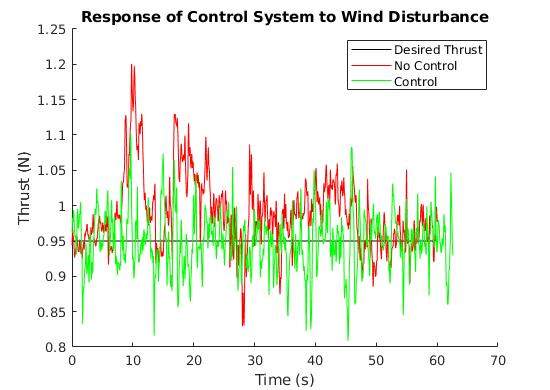
\includegraphics[width=10cm]{images/Figure_2/wind_disturbance.jpg}
	\caption{response}
	\label{wind_disturbance}
\end{figure}

%	\begin{figure}[b]
%	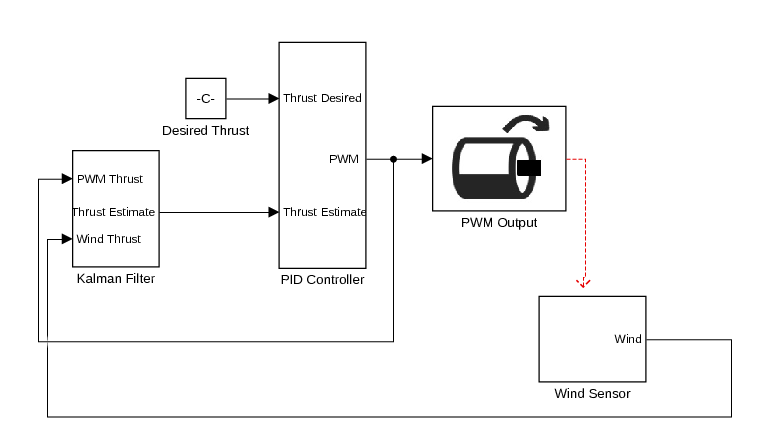
\includegraphics[width=\textwidth / 2]{images/block_diagram.png}
%	\caption{Block Diagram}
%	\label{block_diagram}
%\end{figure}
%	\begin{figure}[b]
%	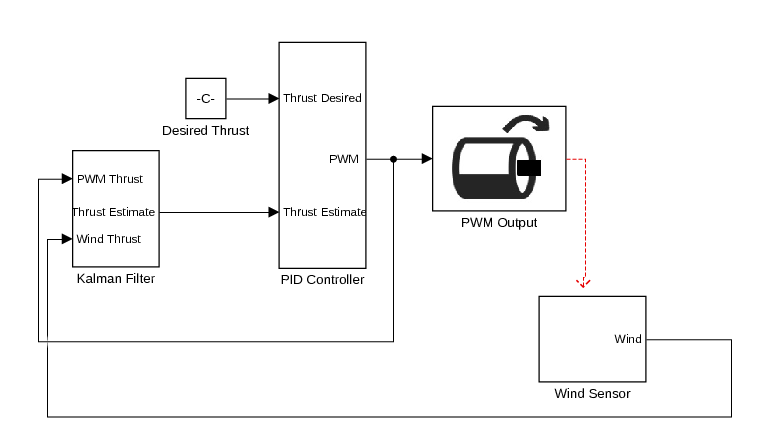
\includegraphics[width=\textwidth / 2]{images/block_diagram.png}
%	\caption{Block Diagram}
%	\label{block_diagram}
%\end{figure}
%	\begin{figure}[b]
%	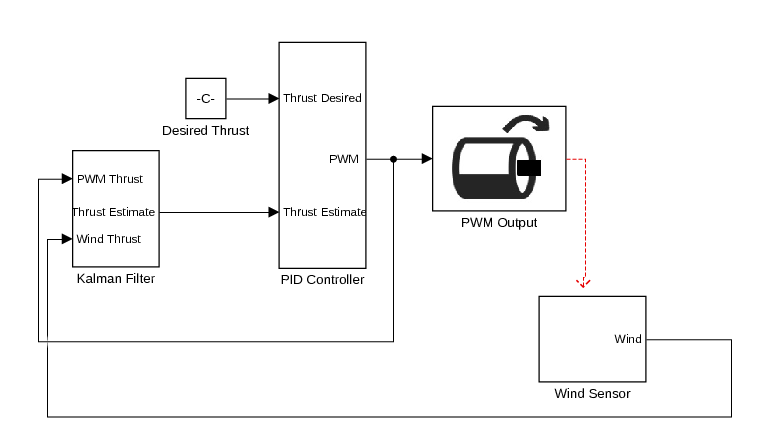
\includegraphics[width=\textwidth / 2]{images/block_diagram.png}
%	\caption{Block Diagram}
%	\label{block_diagram}
%\end{figure}
	
\subsection{5.4}
\begin{thebibliography}{00}
\bibitem{bara}B. J. Emran, D. D. Tannant, and H. Najjaran, “Low-altitude aerial methane concentration mapping,” Remote Sens., vol. 9, no. 8, 2017.
\bibitem{Mathe} K. Máthé and L. Buşoniu, “Vision and Control for UAVs: A Survey of General Methods andof Inexpensive Platforms for Infrastructure Inspection,” Sensors, vol. 15, no. 7, pp. 14887–14916, 2015.
\bibitem{akf} A.H.Mohamed and K. P. Schwarz, “Adaptive Kalman Filtering for INS/GPS,” J. Geod., vol. 73, no. 4, pp. 193–203, 1999.
\bibitem{fuzzy} P. J. Escamilla-Ambrosio and N. Mort, “Development of a fuzzy logic-based adaptive Kalman filter,” in Control Conference (ECC), 2001 European, 2001, pp. 1768–1773.
\bibitem{sebesta} K. D. Sebesta and N. Boizot, “A real-time adaptive high-gain EKF, applied to a quadcopter inertial navigation system,” IEEE Trans. Ind. Electron., vol. 61, no. 1, pp. 495–503, 2014.
\bibitem{Manki} A. Makni, H. Fourati, and A. Y. Kibangou, “Energy-Aware Adaptive Attitude Estimation under External Acceleration for Pedestrian Navigation,” IEEE/ASME Trans. Mechatronics, vol. 21, no. 3, pp. 1366–1375, 2016.
\bibitem{Lin} C. M. Lin and C. S. Hsueh, “Adaptive EKF-CMAC-based multisensor data fusion for maneuvering target,” IEEE Trans. Instrum. Meas., vol. 62, no. 7, pp. 2058–2066, 2013.
\bibitem{Sharman} M. K. Al-Sharman, M. A. Jaradat, and M. F. Abdel-Hafez, “Intelligent attitude and flapping angles estimation of flybarless helicopters under near-hover conditions,” J. Franklin Inst., 2018.
\bibitem{Emran} M. K. Al-Sharman, B. J. Emran, M. A. Jaradat, H. Najjaran, R. Al-Husari, and Y. Zweiri, “Precision landing using an adaptive fuzzy multi-sensor data fusion architecture,” Appl. Soft Comput. J., vol. 69, 2018.
		\bibitem{mahoney1} Mahoney 2012
\bibitem{rcb} https://www.rcbenchmark.com/dynamometer-series-1580/
\bibitem{md} https://moderndevice.com/product/wind-sensor-rev-p/
\bibitem{hot_wire} Extended Applications of the Hot‐Wire Anemometer, Stanley Corrsin,Review of Scientific Instruments 1947 18:7, 469-471 
\bibitem{awan} A. U. Awan, J. Park and H. J. Kim, "Thrust estimation of quadrotor UAV using adaptive observer," 2011 11th International Conference on Control, Automation and Systems, Gyeonggi-do, 2011, pp. 131-136.
\bibitem{sydney} N. Sydney, B. Smyth and D. A. Paley, "Dynamic control of autonomous quadrotor flight in an estimated wind field," 52nd IEEE Conference on Decision and Control, Florence, 2013, pp. 3609-3616.
\end{thebibliography}
\end{document}
